    \documentclass[11pt,
        usenames, % allows access to some tikz colors
        dvipsnames % more colors: https://en.wikibooks.org/wiki/LaTeX/Colors
    ]{article}
    \usepackage{
        amsmath,
        amssymb,
        fouriernc, % fourier font w/ new century book
        fancyhdr, % page styling
        lastpage, % footer fanciness
        hyperref, % various links
        setspace, % line spacing
        amsthm, % newtheorem and proof environment
        mathtools, % \Aboxed for boxing inside aligns, among others
        float, % Allow [H] figure env alignment
        enumerate, % Allow custom enumerate numbering
        graphicx, % allow includegraphics with more filetypes
        wasysym, % \smiley!
        upgreek, % \upmu for \mum macro
        listings, % writing TrueType fonts and including code prettily
        tikz, % drawing things
        booktabs, % \bottomrule instead of hline apparently
        xcolor, % colored text
        cancel % can cancel things out!
    }
    \usepackage[margin=1in]{geometry} % page geometry
    \usepackage[
        labelfont=bf, % caption names are labeled in bold
        font=scriptsize % smaller font for captions
    ]{caption}
    \usepackage[font=scriptsize]{subcaption} % subfigures

    \newcommand*{\scinot}[2]{#1\times10^{#2}}
    \newcommand*{\dotp}[2]{\left<#1\,\middle|\,#2\right>}
    \newcommand*{\rd}[2]{\frac{\mathrm{d}#1}{\mathrm{d}#2}}
    \newcommand*{\pd}[2]{\frac{\partial#1}{\partial#2}}
    \newcommand*{\rdil}[2]{\mathrm{d}#1 / \mathrm{d}#2}
    \newcommand*{\pdil}[2]{\partial#1 / \partial#2}
    \newcommand*{\rtd}[2]{\frac{\mathrm{d}^2#1}{\mathrm{d}#2^2}}
    \newcommand*{\ptd}[2]{\frac{\partial^2 #1}{\partial#2^2}}
    \newcommand*{\md}[2]{\frac{\mathrm{D}#1}{\mathrm{D}#2}}
    \newcommand*{\pvec}[1]{\vec{#1}^{\,\prime}}
    \newcommand*{\svec}[1]{\vec{#1}\;\!}
    \newcommand*{\bm}[1]{\boldsymbol{\mathbf{#1}}}
    \newcommand*{\uv}[1]{\hat{\bm{#1}}}
    \newcommand*{\ang}[0]{\;\text{\AA}}
    \newcommand*{\mum}[0]{\;\upmu \mathrm{m}}
    \newcommand*{\at}[1]{\left.#1\right|}
    \newcommand*{\bra}[1]{\left<#1\right|}
    \newcommand*{\ket}[1]{\left|#1\right>}
    \newcommand*{\abs}[1]{\left|#1\right|}
    \newcommand*{\ev}[1]{\left\langle#1\right\rangle}
    \newcommand*{\p}[1]{\left(#1\right)}
    \newcommand*{\s}[1]{\left[#1\right]}
    \newcommand*{\z}[1]{\left\{#1\right\}}

    \newtheorem{theorem}{Theorem}[section]

    \let\Re\undefined
    \let\Im\undefined
    \DeclareMathOperator{\Res}{Res}
    \DeclareMathOperator{\Re}{Re}
    \DeclareMathOperator{\Im}{Im}
    \DeclareMathOperator{\Log}{Log}
    \DeclareMathOperator{\Arg}{Arg}
    \DeclareMathOperator{\Tr}{Tr}
    \DeclareMathOperator{\E}{E}
    \DeclareMathOperator{\Var}{Var}
    \DeclareMathOperator*{\argmin}{argmin}
    \DeclareMathOperator*{\argmax}{argmax}
    \DeclareMathOperator{\sgn}{sgn}
    \DeclareMathOperator{\diag}{diag\;}

    \colorlet{Corr}{red}

    % \everymath{\displaystyle} % biggify limits of inline sums and integrals
    \tikzstyle{circ} % usage: \node[circ, placement] (label) {text};
        = [draw, circle, fill=white, node distance=3cm, minimum height=2em]
    \definecolor{commentgreen}{rgb}{0,0.6,0}
    \lstset{
        basicstyle=\ttfamily\footnotesize,
        frame=single,
        numbers=left,
        showstringspaces=false,
        keywordstyle=\color{blue},
        stringstyle=\color{purple},
        commentstyle=\color{commentgreen},
        morecomment=[l][\color{magenta}]{\#}
    }

\begin{document}

\section{Laplace Plane Dynamics}

\subsection{Maximum Separatrix Area---Simple}

Consider a planet with orbit normal $\uv{l}_{\rm p}$ that experiences precession
driven by stellar oblateness $\uv{l}_{\rm s}$ and an outer perturber
$\uv{l}_{\rm o}$. We assume that the planet's orbit is circular. The vector
form of the precessional dynamics are (e.g.\ Tremaine+2009, Eq~19):
\begin{align}
    \rd{\uv{l}_{\rm p}}{t}
        &= \omega_{\rm sp} \p{\uv{l}_{\rm p} \cdot \uv{l}_{\rm s}}
            \p{\uv{l}_{\rm p} \times \uv{l}_{\rm s}}
            + \omega_{\rm op} \p{\uv{l}_{\rm p} \cdot \uv{l}_{\rm o}}
            \p{\uv{l}_{\rm p} \times \uv{l}_{\rm o}}.
\end{align}

We first make an important symmetry argument: in the limits of $\omega_{\rm sp}
\ll \omega_{\rm op}$ or $\omega_{\rm sp} \gg \omega_{\rm op}$, the evolution of
$\uv{l}_{\rm p}$ consist of uniform precession about $\uv{l}_{\rm o}$ and
$\uv{l}_{\rm p}$ respectively, and thus the separatrix area must go to zero in
these limits. In fact, the phase portrait must the same under the following
transformation: swap the two frequencies $(\omega_{\rm sp}, \omega_{\rm op})$
and the two vectors $(\uv{l}_{\rm o}, \uv{l}_{\rm s})$. Swapping the precession
frequencies is equivalent to taking $a / r_{\rm M} \mapsto r_{\rm M} / a$ (and
rescaling time), since $\omega_{\rm op} / \omega_{\rm sp} = (a / r_{\rm M})^5$.
Thus, we arrive at an important conclusion: \emph{the phase portraits are
equivalent, up to a rotation of reference frame, for any two $r_{\rm M,1}$ and
$r_{\rm M, 2}$ satisfying $a / r_{\rm M, 1} = r_{\rm M, 2} / a$}. This implies
that the separatrix area is symmetric about $r_{\rm M} = a$ as well.

It's not clear that the separatrix area must be monotonic between $r_{\rm M} \in
\s{0, a}$, but intuitively \textbf{this seems like it should be the case} (?),
since there are no special values of $\omega_{\rm sp} / \omega_{\rm op}$ in the
equation of motion. If so, then the maximum separatrix area is obtained for
$r_{\rm M} = a$. The curve for the separatrix in this case is significantly
easier to obtain, though it still seems difficult to integrate explicitly (maybe
there's a clever idea?).

To compute the separatrix area for $a = r_{\rm M}$, we note that the
low-obliquity Laplace equilibrium P1 is located exactly halfway between
$\uv{l}_{\rm o}$ and $\uv{l}_{\rm s}$. Thus, we choose the reference frame such
that $\uv{z}\propto \uv{l}_{\rm o} + \uv{l}_{\rm s}$, and we choose $\uv{y}$ to
point towards P2 (which is always $\pi/2$ away from P1). Then, defining
\begin{equation}
    \cos \epsilon \equiv \uv{l}_{\rm o} \cdot \uv{l}_{\rm s},
\end{equation}
we can write
\begin{align}
    \uv{l}_{\rm o} &= \cos \frac{\epsilon}{2} \uv{z} + \sin
        \frac{\epsilon}{2}\uv{x},\\
    \uv{l}_{\rm s} &= \cos \frac{\epsilon}{2} \uv{z} - \sin
        \frac{\epsilon}{2}\uv{x}.
\end{align}
Finally, upon inspection, $\uv{x}$ is also an equilibrium point, which must be
P3. \textbf{In summary, in this reference frame, P1 lies along $\uv{z}$, P2 lies
along $\uv{y}$, and P3 lies along $\uv{x}$}.

To get the level curve corresponding to the separatrix, we evaluate the
Hamiltonian (factoring out the prefactor $\omega_{\rm sp} = \omega_{\rm op}$)
and adopt a spherical coordinate system:
\begin{align}
    H &\propto -\frac{1}{2} \s{
        \p{\uv{l}_{\rm p} \cdot \uv{l}_{\rm s}}^2
        + \p{\uv{l}_{\rm p} \cdot \uv{l}_{\rm o}}^2},\\
    \tilde{H}\p{\theta, \phi} &= -\s{
        \sin^2\frac{\epsilon}{2}\sin^2\theta\cos^2\phi
        + \cos^2\frac{\epsilon}{2} \cos^2\theta},
\end{align}
where we have adopted spherical coordinates $(\theta, \phi)$ to describe the
orientation of $\uv{l}_{\rm p}$, and $\theta = \pi/2, \phi = 0$ corresponds to
$\uv{x}$. We first evaluate $H$ (dropping the tilde) at P3:
\begin{equation}
    H_3 = -\sin^2\frac{\epsilon}{2},
\end{equation}
then the separatrix is given by
\begin{align}
    H\p{\theta_{\rm sep}(\phi), \phi} &= H_3,\\
    \sin^2\frac{\epsilon}{2}\p{1 - \cos^2\theta_{\rm sep}}\cos^2\phi
        + \cos^2\frac{\epsilon}{2} \cos^2\theta_{\rm sep}
        &= \sin^2\frac{\epsilon}{2},\\
    \cos^2\theta_{\rm sep} &= \frac{\sin^2\frac{\epsilon}{2}\sin^2\phi}{
            \cos^2\frac{\epsilon}{2} -
            \sin^2\frac{\epsilon}{2}\cos^2\phi}\nonumber\\
        &= \frac{\sin^2\phi}{\cot^2\frac{\epsilon}{2} - \cos^2\phi},\\
    A_{\rm sep} &= 4\int\limits_0^\pi \cos_+\theta_{\rm sep}\;\mathrm{d}\phi.
\end{align}
Here, $\cos_+\theta_{\rm sep}$ indicates that we take the positive root; one
factor of two arises because the vertical extent of the separatrix is
$\cos_+\theta_{\rm sep} - \cos_- \theta_{\rm sep}$, and a second factor of two
arises because we are only integrating $\phi \in [0, \pi]$. Under this
convention, the maximum possible phase space area is $4\pi$. We display the
value of $A_{\rm sep}$ in Fig.~\ref{fig:laplace}.
\begin{figure}
    \centering
    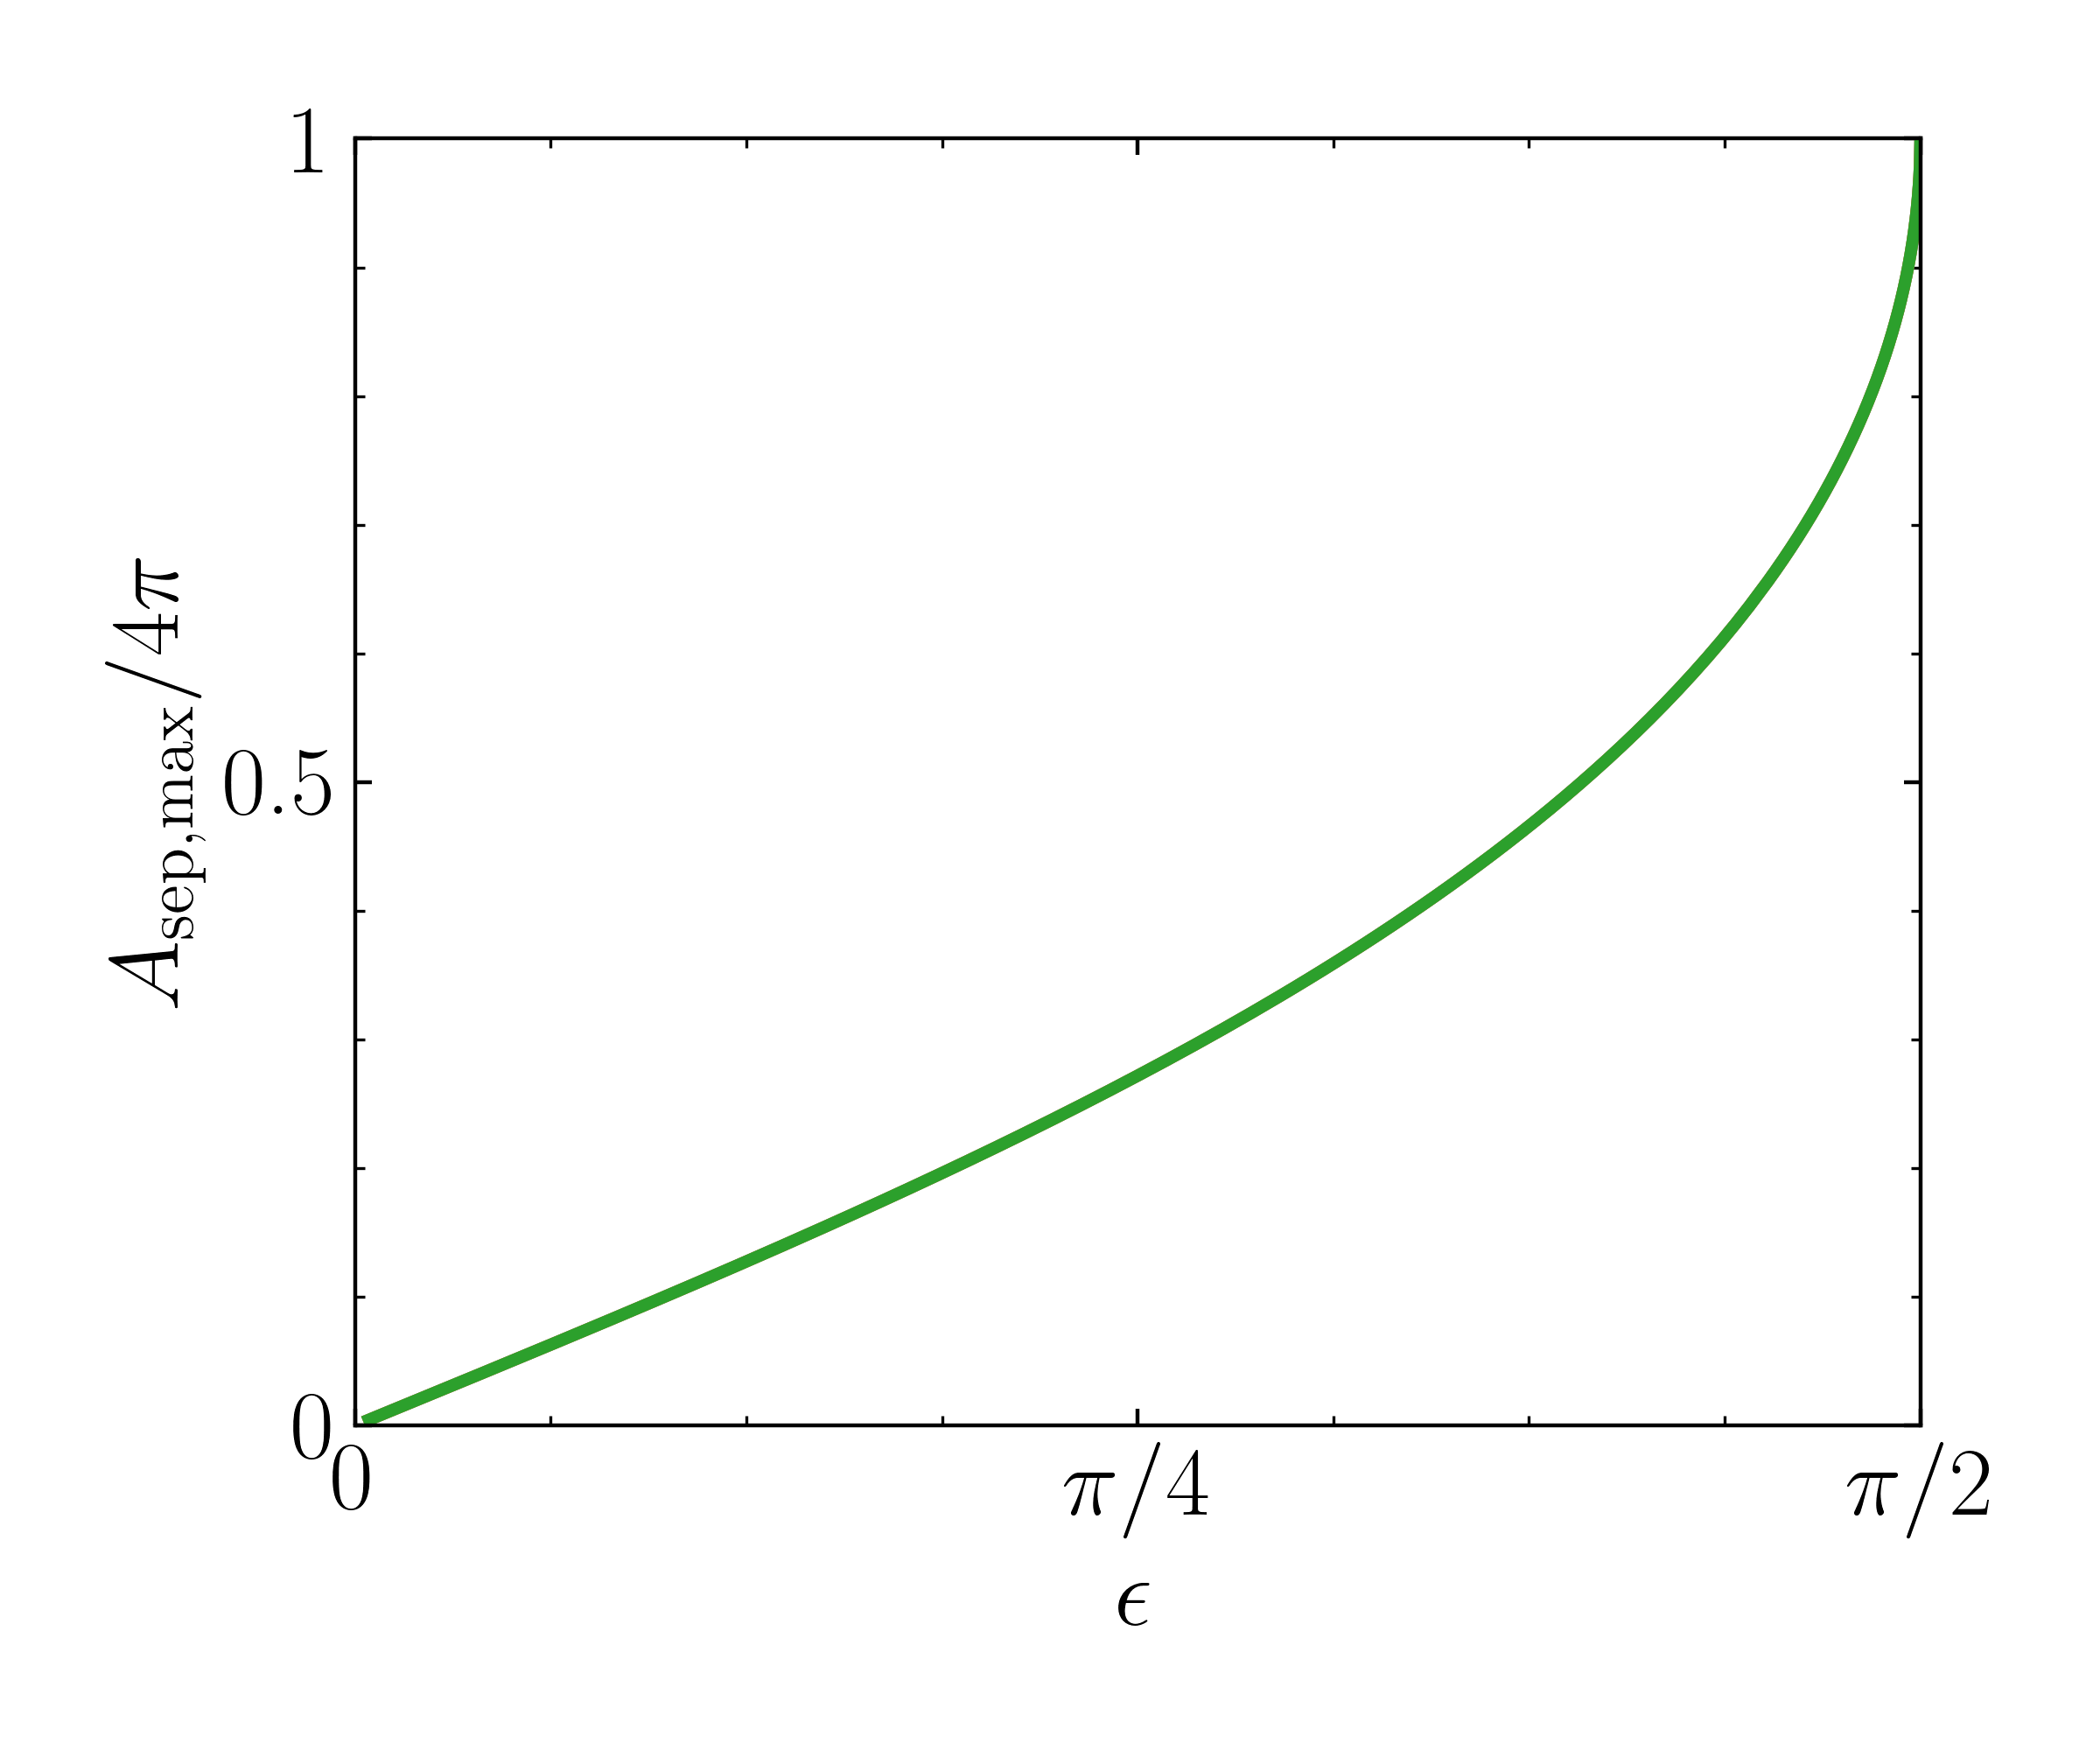
\includegraphics[width=0.5\columnwidth]{laplace.png}
    \caption{Fractional phase space area enclosed by the maximal separatrix as a
    function of $\epsilon$. Reminder: this is the area surrounding Laplace
    equilibrium P2 when $r_{\rm M} = a$, which is also the maximum extent of the
    separatrix.}\label{fig:laplace}
\end{figure}

Note: the integral for $A_{\rm sep}$ is analytic:
\begin{align}
    A_{\rm sep} &= 4\int\limits_0^\pi
            \frac{\sin\phi}{\sqrt{\cot^2\frac{\epsilon}{2} - \cos^2\phi}}
            \;\mathrm{d}\phi\nonumber\\
        &= 4\int\limits_{-1}^1
            \frac{1}{\sqrt{\cot^2\frac{\epsilon}{2} - \cos^2\phi}}
            \;\mathrm{d}\cos \phi\nonumber\\
        &= 4\s{\tan^{-1}\p{\frac{u}{
            \sqrt{\cot^2\frac{\epsilon}{2} - u^2}}}}_{u=-1}^{u=1}\nonumber\\
        &= 8\s{\tan^{-1}\sqrt{\frac{\sin^2(\epsilon / 2)}{\cos \epsilon}}}.
\end{align}

\subsection{Maximum Separatrix Area---Melaine}

Melaine says that the separatrix is given by the solutions to the equation
($I_Q$ is the satellite inclination to the planet equator, and $\delta Q$ is the
corresponding phase angle; we call these $\theta,\phi$ above)
\begin{align}
    \tan I_{\rm Q,\pm}
        &= \frac{\cos \delta Q \sin (2\epsilon) \pm \sin \delta Q
            \sin \epsilon\sqrt{2\p{u - 1 + \sqrt{1 + u^2 + 2u\cos\p{2\epsilon}}}}}{
            u + 1 - 2\cos^2 \delta Q \sin^2\epsilon - \sqrt{1 + u^2 +
            2u\cos(2\epsilon)}}.
\end{align}
Here $u = r_{\rm M}^5/a^5$.
However, this expression is singular for $\cos \delta_Q = w_{\pm}$, where
\begin{equation}
    w_{\pm} = \pm \sqrt{\frac{1 + u - \sqrt{1 + u^2 +
        2u\cos(2\epsilon)}}{2\sin^2\epsilon}}.
\end{equation}
This is where the denominator vanishes. Note that this must be a
removable/coordinate singularity: physically, there is no special value of
$\delta_Q$. The separatrix area is then just given by integrating $\cos I_Q$ but
taking the correctly-signed roots, which Melaine works out to be
\begin{align}
    \frac{A}{2} ={}&
            \int\limits_0^\pi \cos I_{\rm Q, +} - \cos I_{\rm Q,
            -}\;\mathrm{d}\delta_Q,\\
        ={}&
        \int\limits_0^{\arccos w_+}
            \p{\frac{-1}{\sqrt{1 + x_+^2}}
                - \frac{-1}{1 + x_-^2}}\;\mathrm{d}\delta_Q\nonumber\\
        &+ \int\limits_{\arccos w_+}^{\arccos w_-}
            \p{\frac{1}{\sqrt{1 + x_+^2}}
                - \frac{-1}{1 + x_-^2}}\;\mathrm{d}\delta_Q\nonumber\\
        &+ \int\limits_{\arccos w_-}^{\pi}
            \p{\frac{1}{\sqrt{1 + x_+^2}}
                - \frac{1}{1 + x_-^2}}\;\mathrm{d}\delta_Q.
\end{align}

We find that the two expressions agree, see Fig.~\ref{fig:laplace}. Is it
obvious that they should? Setting $u = 1$, we find that
\begin{align}
    \tan I_{\rm Q, \pm} &=
        \frac{\cos \delta Q \sin (2\epsilon) \pm \sin \delta Q
            \sin \epsilon\sqrt{4\cos \epsilon}}{
            2 - 2\cos^2 \delta Q \sin^2\epsilon - 2\cos \epsilon}\nonumber\\
        &=
        \frac{\cos \delta Q \sin (2\epsilon) \pm \sin \delta Q
            \sin \epsilon\sqrt{4\cos \epsilon}}{
            2 - 2\cos^2 \delta Q \sin^2\epsilon - 2\cos \epsilon}.
\end{align}
Not obvious.

\clearpage

\section{Constraints on Perturber}

For the mechanism to work, we need a host star with mass $m_\star$ and a
distant perturber with mass $m_2$.
We will denote the planet's properties with $p$ subscripts.

In order for the mechanism to work, we need to know the Laplace radius of the
star as it spins down.
This is easy to do by generalizing the expression in my paper with Melaine.
The Laplace radius should be:
\begin{align}
    r_{\rm M}^5
        &=
            \frac{2k_{2,\star}}{3}
                \frac{m_\star + m_2}{m_2}
                \p{\frac{\omega_\star}{n_b}}^2
                R_\star^5,\\
% >>> (2 * 0.02 / 3 * 2 * ((2 * pi / (3 day))^2 / (G * (2 Msun) / (300 AU)^3)) * Rsun^5)^(1/5) / au
% 0.410014
    r_{\rm M}
        &= 0.41\;\mathrm{au}
            \p{\frac{k_2}{0.02}}^{1/5}
            \p{\frac{\omega_\star}{2\pi / \p{3\;\mathrm{day}}}}^{2/5}
            \p{\frac{m_2}{M_{\odot}}}^{-1/5}
            \p{\frac{a_{\rm b}}{300\;\mathrm{AU}}}^{3/5}
            \p{\frac{R_\star}{R_{\odot}}}.
\end{align}
Here, b subscripts denotes properties of the binary, and we've taken $m_\star =
m_2 = M_{\odot}$.
Thus, if a star spins down by $10\times$, its Laplace radius migrates by
$10^{2/5} \approx 2.5$, or $r_{\rm M} \sim 0.16\;\mathrm{au}$.
For reference, a planet on a $10\;\mathrm{day}$ orbit (typical of polar
Neptunes) is located at $\sim 0.1\;\mathrm{au}$.
% >>> (G * Msun / (2 * pi / (10 day))^2)^(1/3) / au
% 0.090844

In order for this mechanism to work, we really need to be looking at stellar
companions a factor of $\sim 10 \times$ closer, since $10^{3/5} \sim 4$, so that
it sweeps through the $0.1\;\mathrm{au}$ range.
Moreover, considering that high-e migration typically circularizes the planet at
$\sim 3\;\mathrm{day}$ (a few times the tidal radius $R_{\rm p} / (M_\star /
m_{\rm p})^{1/3} \sim 0.01\;\mathrm{au}$), the Laplace plane transition will
generally struggle to do much for post-high-e-migration.

However, interestingly, if we consider instead CJ companions:
\begin{equation}
% >>> (2 * 0.02 / 3 * 2 * ((2 * pi / (3 day))^2 / (G * (Mjup) / (5 AU)^3)) * Rsun^5)^(1/5) / au
% 0.162249
    r_{\rm M}
        = 0.16\;\mathrm{au}
            \p{\frac{k_2}{0.02}}^{1/5}
            \p{\frac{\omega_\star}{2\pi / \p{3\;\mathrm{day}}}}^{2/5}
            \p{\frac{m_2}{M_{\rm J}}}^{-1/5}
            \p{\frac{a_{\rm b}}{5\;\mathrm{AU}}}^{3/5}
            \p{\frac{R_\star}{R_{\odot}}}.
\end{equation}
Thus, a CJ misaligned from an inner Neptune may introduce nontrivial Laplace
plane transitions.
Such a mechanism naturally arises from Petrovich+20, the current (only?) favored
mechanism for polar Neptunes.
However, if there is just primordial disk misalignment, then as the star spins
down, the SE+CJ systems may experience this transition.
Of course, there is no preferennce for $90^\circ$ once the star spins down, and
since there is no dissipation, we should roughly have $\theta_{\rm \star-p, i}
\sim \theta_{\rm p-CJ, f}$.
But the obliquity will broadly oscillate!

\clearpage

\subsection{ZLK and Laplace Plane Transition Parameter Space}

If we want the planet to undergo high-eccentricity migration via the ZLK +
tides mechanism, then it will circularize no closer\footnote{It can circularize
wider, if the eccentricity is so extreme that the eccentricity tide circularize
the orbit before $a_{\rm  peri, \min}$ is reached, and it may not circularize at
all, if the pericenter distance is too large to give efficient tidal
dissipation.} than $\simeq 2a_{\rm peri, \min}$, where $a_{\rm peri, \min}$ is
set by the combination of ZLK and short range forces.
This is because orbital AM ($\propto \sqrt{a(1 - e^2)}$) is conserved by the
eccentricity tide (driven by the pseudosynchronously-spinning planet).

We can express $a_{\rm peri, \min}$ in terms of $j_{\min} \equiv \sqrt{1 -
e_{\max}^2}$
\begin{align}
    a_{\rm peri, \min}
        &=
            aj_{\min},
\end{align}
where $j_{\min}$ satisfies (Liu, Munoz \& Lai 2015, with $m_\star + m_{\rm p}
\approx m_\star$ taken)
\begin{align}
        \frac{9}{8}e_{\max}^2 &=
        \frac{\epsilon_{\rm tide}}{15}
            \p{\frac{1 + 3e_{\max}^2 + \tfrac{3e_{\max}^4}{8}}{j_{\min}^9} - 1}
        +
        \frac{\epsilon_{\rm rot}}{3}
            \p{\frac{1}{j_{\min}^3} - 1}
        +
        \epsilon_{\rm GR} \p{\frac{1}{j_{\min}} - 1},\\
        \label{eq:emax_srfs}
    \epsilon_{\rm GR}
        &= \frac{3Gm_{\star}^2 a_{\rm out}^3}{a^4c^2m_2},\\
    \epsilon_{\rm tide}
        &= \frac{15 m_{\rm p}
            a_{\rm out}^3 k_{2,\star}R_\star^5}{
                a^8 m_2},\\
    \epsilon_{\rm rot}
        &=
            \frac{a_{\rm out}^3\,
                k_{2,\star}R_\star^5}{2Ga^5 m_2}
                \omega_{\rm \star}^2\nonumber\\
        &=
            \frac{(m_\star + m_2)
                k_{2,\star}R_\star^5}{2a^5 m_2}
                \p{\frac{\omega_{\rm \star}}{n_{\rm out}}}^2,
\end{align}
where the host star uses $\star$ subscripts, the planet $p$, and the
perturbing/binary companion $2$; $a$ is the sma of the inner binary, and
$a_{\rm out}$ refers to that of the outer binary (which we take to be circular
for convenience).

For young stellar hosts, which are typically rotating rapidly, $\epsilon_{\rm
rot}$ dominates the short range force contributions.
Taking $e_{\max} \approx 1$, we obtain
\begin{align}
    \frac{9}{8} &\approx \frac{\epsilon_{\rm rot}}{3j_{\min}^3},\\
    j_{\min} &\approx
        \frac{2}{3}\epsilon_{\rm rot}^{1/3},\\
    \frac{a_{\rm peri, \min}}{a}
        &\approx \frac{2}{3}\epsilon_{\rm rot}^{1/3},\\
    \frac{a_{\rm peri, \min}}{R_\star}
        &=
            \frac{2}{3}
            \p{\frac{(m_\star + m_2)k_{2,\star}}{2m_2}}^{1/3}
            \p{\frac{R_\star}{a_0}}^{2/3}
            \p{\frac{\omega_{\rm \star, 0}}{n_{\rm out}}}^{2/3},
\end{align}
where we have denoted $\omega_{\rm \star, 0}$ to point out that $a_{\rm peri,
\min}$ is set by the star's early spin rate, and $a_0$ to remind us that this is
the \emph{starting} sma of the planet.

As such, we need $r_{\rm M}$, the Laplace radius, to cross $2a_{\rm peri, \min}$,
where:
\begin{align}
    \frac{r_{\rm M, [0, f]}}{R_\star}
        &=
            \p{\frac{2k_{2,\star}}{3}
                \frac{m_\star + m_2}{m_2}}^{1/5}
                \p{\frac{\omega_{\rm \star,[0, f]}}{n_{\rm out}}}^{2/5}
                ,
\end{align}
where the subscripts $0, f$ denote the dependence of the initial/final
Laplace radii on the initial/final stellar spin frequency.
The hierarchy demanded by our scenario is, to be explicit:
{\small
\begin{align}
    \p{\frac{2k_{2,\star}}{3}
        \frac{m_\star + m_2}{m_2}}^{1/5}
        \p{\frac{\omega_{\rm \star,f}}{n_{\rm out}}}^{2/5}
        &<
            \frac{4}{3}
            \p{\frac{(m_\star + m_2)k_{2,\star}}{2m_2}}^{1/3}
            \p{\frac{R_\star}{a_0}}^{2/3}
            \p{\frac{\omega_{\rm \star, 0}}{n_{\rm out}}}^{2/3}
        <
    \p{\frac{2k_{2,\star}}{3}
        \frac{m_\star + m_2}{m_2}}^{1/5}
        \p{\frac{\omega_{\rm \star,0}}{n_{\rm out}}}^{2/5},\\
    \p{\frac{\omega_{\rm \star,f}}{\omega_{\rm \star,0}}}^{2/5}
        &<
            \frac{4}{3}
            \p{\frac{3}{2}}^{1/5}
            \p{\frac{1}{2}}^{1/3}
            \p{\frac{R_\star}{a_0}}^{2/3}
            \p{\frac{k_{2,\star}(m_\star + m_2)}{m_2}}^{2/15}
            \p{\frac{\omega_{\rm \star, 0}}{n_{\rm out}}}^{4/15}
        <
    1.\label{eq:constr}
\end{align}}
The key quantity to evaluate then is the middle quantity:
\begin{align}
    \frac{2a_{\rm peri, \min}}{r_{\rm M, 0}}
        &\approx
% >>> 4/3 * (3/2)^(1/5) * (1/2)^(1/3) * (Rsun / AU)^(2/3) * (0.04 * 2)^(2/15) * ((2 * pi / (3 day)) / (G * (2 Msun) / (100 AU)^3)^(1/2))^(4/15)
% 0.472549
        0.5
            \p{\frac{R_\star}{R_{\odot}}}^{2/3}
            \p{\frac{a_0}{\mathrm{au}}}^{-2/3}
            \p{\frac{\omega_{\star, 0}}{2\pi / (3\;\mathrm{day})}}^{4/15}
            \p{\frac{(m_\star + m_2) / m_2}{2}}^{2/15}
            \p{\frac{a_{\rm out}}{100\;\mathrm{au}}}^{2/5}.
\end{align}
We've also taken $m_{\star} = m_2 = M_{\odot}$ and $k_{2,\star} = 0.04$, typical
for Sun-like stars.

Recalling that spindown can take us from $3\;\mathrm{day}$ to $30\;\mathrm{day}$
spin periods, roughly, the quantity on the left hand side of
Eq.~\eqref{eq:constr} evaluates to
\begin{equation}
    \p{\frac{\omega_{\rm \star,f}}{\omega_{\rm \star,0}}}^{2/5}
        \simeq 0.4.
\end{equation}
So for the fiducial parameters above, the required hierarchy of scales works:
$r_{\rm M}$ will indeed sweep through the location of the planet's present-day
semi-major axis ($\simeq 2a_{\rm peri, \min}$).

Of course, this is all conditional on the requirement that $a_{\rm peri, \min}$
be close-in enough to induce merger.
Using the standard planetary equilibrium tide, (e.g.\ Leconte+2010) and taking
$e \to 1$, we obtain
\begin{align}
    \rd{\ln a}{t}
        &\sim
            \frac{3k_{\rm 2p}}{Q}
            \frac{M_\star}{M_{\rm p}}
            \p{\frac{R_{\rm p}}{a}}^5 n
            \frac{231}{480\p{1 - e}^6},\\
% >>> 1 / (3 * 0.3 / 1e3 * Msun / Mneptune * (Rneptune / (0.06 AU))^5 * (G * Msun / ((1 AU) * (0.06 AU)^2))^(1/2) * (231/480)) / yr
% 7.279403e+09
        &\sim
            \frac{1}{8\;\mathrm{Gyr}}
            \p{\frac{a_{\rm peri}}{0.06\;\mathrm{au}}}^{-6}
            \p{\frac{a}{\mathrm{au}}}^{-1/2}
            \p{\frac{M_\star / M_{\rm p}}{M_{\odot} / M_{\rm Nep}}}
            \p{\frac{k_{\rm 2p} / Q}{0.3 / 10^3}}
            \p{\frac{R_{\rm p}}{R_{\rm Nep}}}^{5}.
\end{align}
This can be helped somewhat by using that $R_{\rm p}$ likely larger for young
planets, and may also be inflated by tidal heating.

\end{document}

